We  will now describe an explicit attack against the NIPoPoW suffix proof construction under a velvet fork. Note that since the protocol is implemented under a velvet fork, any adversarial block that is mined in the proper way except containing false interlink data structure will be accepted as valid. A false interlink may contain invalid pointers, for example pointers to superblocks of a fork chain, as shown in Figure \ref{fig:false_interlink}.
Taking advantage of this fact, an adversary maintaining a fork chain could produce suffix proofs that claim blocks of the chain adopted by an honest player as her own. The attack is described in detail in the following.

\begin{figure}[h]
	\begin{center}
		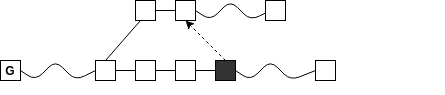
\includegraphics[scale=0.6]{figures/false_interlink.png}
	\end{center}
	\caption{\textit{Example of false interlink structure of an adversarial block, coloured black, in an honest player's chain. The dashed arrow is a pointer to a fork chain superblock included in the interlink.}}
	\label{fig:false_interlink}
\end{figure}

Assume that chain $C_B$ was adopted by an honest player B and chain $C_A$, a fork of $C_B$ at some block, maintained by an adversary A. Assume the adversary wants to produce a suffix proof in order to attack an honest light client to have him adopt chain $C_A$. In order to achieve this, the adversary needs to include a greater amount of PoW in her suffix proof, $\pi_A$, in comparison to the honest player's proof, $\pi_B$, so as to achieve $\pi_A \geq_m \pi_B$. For this she produces some blocks in chains $C_A$ and $C_B$ containing false interlink pointers which will allow for claiming blocks of chain $C_B$ as of chain $C_A$ in her suffix proof.

The general setting of this attack is represented in Figure \ref{fig:generic_attack}. The dashed arrows represent interlink pointers of some level $\mu_A$. Starting from the most recently mined block in the adversary's fork chain and following the interlink pointers a chain is formed which consists the adversary's suffix proof. Blocks of both chains are included in this proof and a verifier could not distinguish the false interlink pointers forming this chain proof and, as a result, would consider it a valid proof. 

\begin{figure}[h]
	\begin{center}
		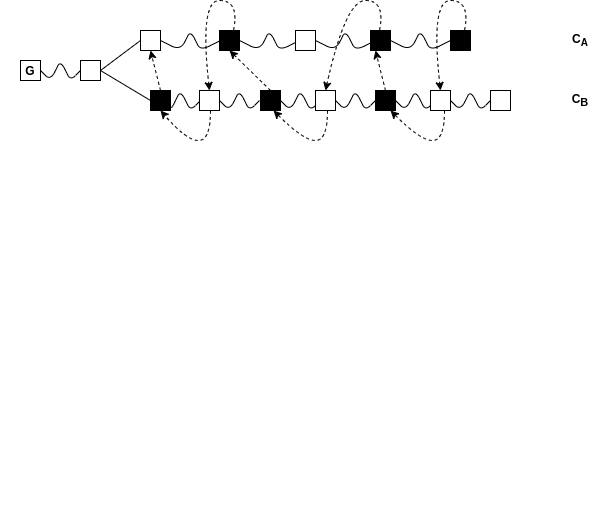
\includegraphics[scale=0.55]{figures/generic_chainsewing_attack.png}
	\end{center}
	\caption{\textit{Generic Chainsewing Attack. $C_B$ is the chain of an honest player and $C_A$ the adversary's chain. Blocks generated by the adversary are colored black. Dashed arrows represent interlink pointers included in the adversary's suffix proof. Wavy lines imply one or more blocks.}}
	\label{fig:generic_attack}
\end{figure}

As the generic attack scheme may seem a bit complicated we will now describe a more specific attack case. Consider that the adversary acts as described below. 
Assume that the adversary chooses to attack at some level $\mu_A$. As shown in Figure \ref{fig:attack} she first generates a superblock $b'$ in her fork chain $C_A$ and a superblock $a'$ in the honest chain $C_B$ which are connected via an invalid interlink pointer from $a'$ to $b'$. As argued earlier, block $a'$ will be accepted as valid in the honest chain $C_B$ despite the false pointers in the interlink data structure. After that the adversary may mine on chain $C_A$ or $C_B$, or not mine at all. At some point she produces a block $a$ in $C_A$ containing an interlink pointer to a block $b$ of the honest player's chain $C_B$. Because of the way blocks are generated by updated honest miners there will be successive interlink pointers leading from block $b$ to block $a'$. Thus following the interlink pointers a chain is formulated which connects $C_A$ blocks $a$ and $b'$ and contains an arbitrarily large part of the honest player's chain $C_B$.

At this point the adversary will produce a suffix proof for chain $C_A$ containing the subchain $C\{ab\} \cup C\{b:a'\} \cup C\{a':b'\}$. Notice that following the interlink pointers constructed in such a way, a light client perceives $C\{ab\} \cup C\{b:a'\} \cup C\{a':b'\}$  as a valid chain.

\begin{figure}[h!]
	\begin{center}
		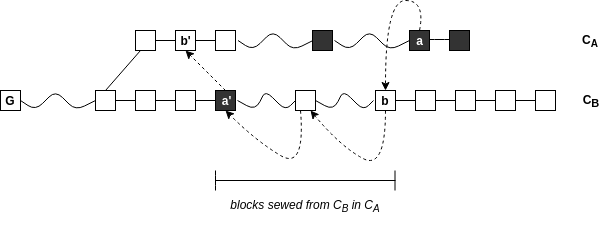
\includegraphics[scale=0.55]{figures/chainsewing_attack.png}
	\end{center}
	\caption{\textit{Chainsewing Attack. The chain at the bottom represents the chain of an honest player, $C_B$, while the above one is the adversarial fork, $C_A$. Blocks generated by the adversary are colored black. Dashed arrows represent interlink pointers included in the suffix proof by the adversary. Wavy lines imply one or more blocks. Firm lines imply the previousId relationship between two sequential blocks.}}
	\label{fig:attack}
\end{figure}

In this attack the adversary uses false interlink pointers to ``sew`` portions of the chain adopted by an honest player to her own fork. This remark justifies the name given.  

Note that in order to make this attack successful, the adversary has to produce only a few superblocks which let her arrogate an arbitrary large number of blocks of an honest player's chain, while she can mine for her own fork chain. Thus intuitively we expect this attack to succeed with overwhelming probability.

@TODO

Needs to be proven. It is not obvious that the attacker will succeed in high probability, since the most important adversarially generated blocks , $a$ and $a'$, set a limit to the adversarial blocks produced in parallel to the honest blocks of subchain $C\{ab\} \cup C\{b:a'\} \cup C\{a':b'\}$ and can take part in the suffix proof.
